%----------------------------------------------------------------------------------------
%    PACKAGES AND THEMES
%----------------------------------------------------------------------------------------

\documentclass[aspectratio=169,xcolor=dvipsnames]{beamer}
\usetheme{SimpleDarkBlue}

\usepackage{hyperref}
\usepackage{graphicx} % Allows including images
\usepackage{booktabs} % Allows the use of \toprule, \midrule and \bottomrule in tables

%----------------------------------------------------------------------------------------
%    TITLE PAGE
%----------------------------------------------------------------------------------------

\title{Multi-core scheduling}
\subtitle{Performance Evaluation of Computer Systems and Networks project}

\author{Taulant Arapi (645308)\\Francesco Barcherini (645413)\\Antonio Ciociola (645324)}
\date{\today} % Date, can be changed to a custom date

%----------------------------------------------------------------------------------------
%    PRESENTATION SLIDES
%----------------------------------------------------------------------------------------

\begin{document}

\begin{frame}
    % Print the title page as the first slide
    \titlepage
\end{frame}

%------------------------------------------------

\begin{frame}{Queueing system modelling}
    \begin{columns}[c]
        \column{.55\textwidth}
        \begin{itemize}
            \item Ready queue: $M/M/C$ queue, $C = N$ CPUs
            \item I/O phase: $M/M/\infty$ queue
            \item Parameters:
            \begin{itemize}
                \item $\gamma_1 = \frac{1}{E[T]}$: process generation rate
                \item $\pi_0 = \pi_1 = \frac{1}{2}$: routing probabilities
                \item $\mu_{cpu} = \frac{1}{E[t_{cpu}]}$, $\mu_{io} = \frac{1}{E[t_{io}]}$
                \item $\rho = \frac{\lambda_1}{N\mu_{cpu}}$, where $\lambda_1 = \frac{2}{E[T]}$: CPU utilization
            \end{itemize}
            \item System is stable if $N > \frac{3p+1}{5}\cdot \frac{E[D]}{E[T]}$
            \item Metrics:
            \begin{itemize}
                \item Turnaround time
                \item Waiting time
                \item CPU utilization
                \item Ready queue length
            \end{itemize}
        \end{itemize}
        \column{.4\textwidth}
        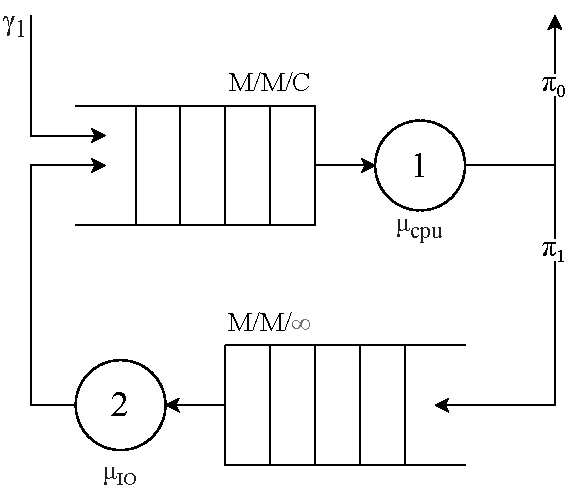
\includegraphics[width=\textwidth]{files/queue_schema.pdf}
    \end{columns}
\end{frame}

%------------------------------------------------

\begin{frame}{OMNeT++ model}
    \begin{columns}[c] % The "c" option specifies centered vertical alignment while the "t" option is used for top vertical alignment

    \column{.45\textwidth} % Left column and width
    \begin{itemize}
        \item Process generator: exponential inter-arrival time and duration
        \item Scheduler: infinite FIFO queue or priority queue (FCFS/SJF)
        \item CPU: $N$ of them (4 or 12)
    \end{itemize}

    \column{.45\textwidth} % Right column and width
    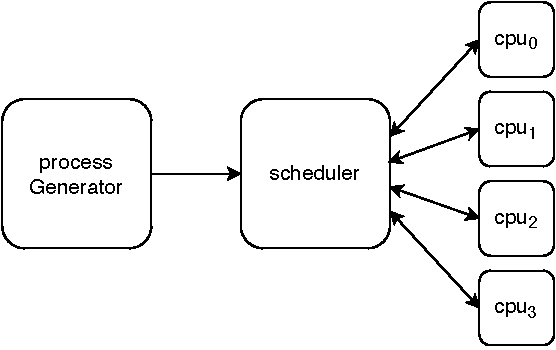
\includegraphics[width=\textwidth]{files/Computer.pdf} % oppure files/sim_schema.png
\end{columns}
    
\end{frame}

%------------------------------------------------

\begin{frame}{Warm-up and Simulation Time}
    \begin{columns}[c]
        \column{.95\textwidth}
        Use number of busy CPUs (out of $N = 4$) as metric.
    \end{columns}
    \begin{columns}[c] % The "c" option specifies centered vertical alignment while the "t" option is used for top vertical alignment
        \column{.45\textwidth} % Left column and width
        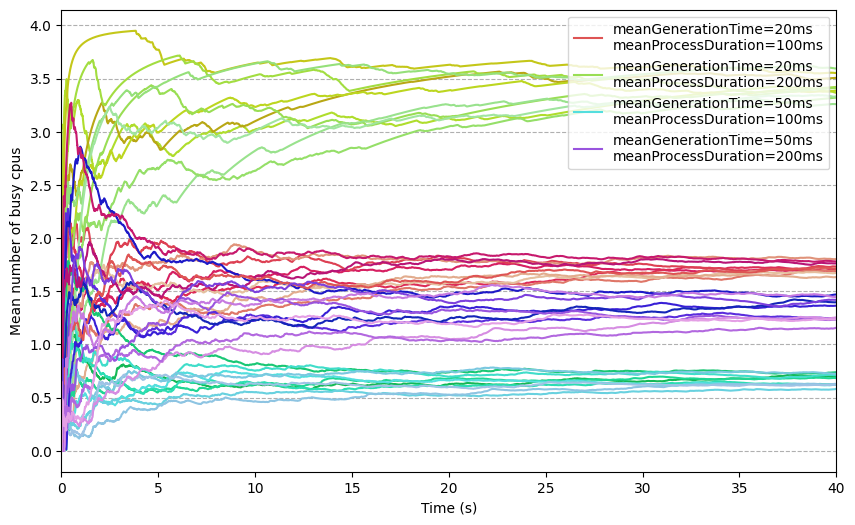
\includegraphics[width=\textwidth]{files/report_images_04/lineWarmup.png}
        \column{.45\textwidth} % Right column and width
        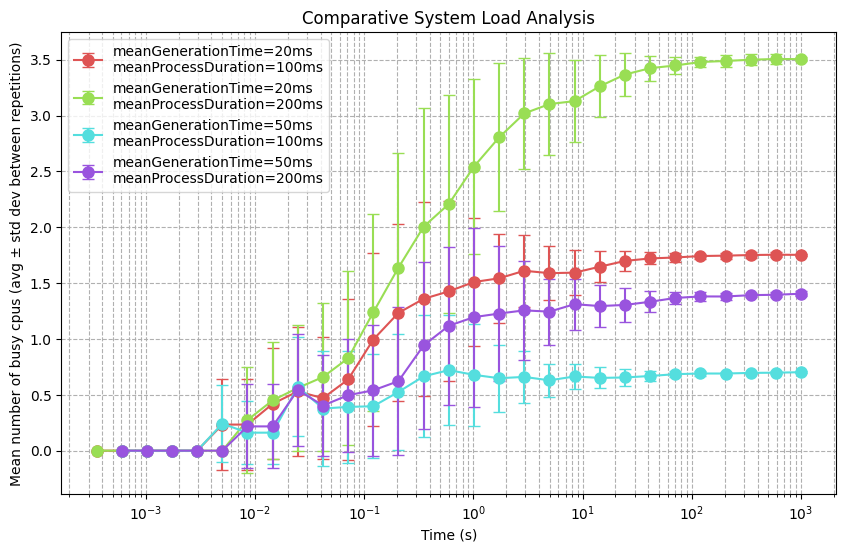
\includegraphics[width=\textwidth]{files/report_images_04/errorWarmup.png}
    \end{columns}
    \begin{columns}[c]
        \column{.6\textwidth}
        \begin{block}{}
            Chosen warm-up time: 200 s\\
            Chosen simulation time: 800 s (excluding warm-up time)
        \end{block}
        \column{.3\textwidth}
    \end{columns}
\end{frame}

%------------------------------------------------

\begin{frame}{Casi particolari?}
    \begin{columns}[c] % The "c" option specifies centered vertical alignment while the "t" option is used for top vertical alignment

        \column{.45\textwidth} % Left column and width
        \textbf{Heading}
        \begin{enumerate}
            \item Statement
            \item Explanation
            \item Example
        \end{enumerate}

        \column{.45\textwidth} % Right column and width
        Lorem ipsum dolor sit amet, consectetur adipiscing elit. Integer lectus nisl, ultricies in feugiat rutrum, porttitor sit amet augue. Aliquam ut tortor mauris. Sed volutpat ante purus, quis accumsan dolor.

    \end{columns}
\end{frame}

%------------------------------------------------

\begin{frame}{Table}
    \begin{table}
        \begin{tabular}{l l l}
            \toprule
            \textbf{Treatments} & \textbf{Response 1} & \textbf{Response 2} \\
            \midrule
            Treatment 1         & 0.0003262           & 0.562               \\
            Treatment 2         & 0.0015681           & 0.910               \\
            Treatment 3         & 0.0009271           & 0.296               \\
            \bottomrule
        \end{tabular}
        \caption{Table caption}
    \end{table}
\end{frame}

%------------------------------------------------

\begin{frame}{Statistiche statistiche}
    Uncomment the code on this slide to include your own image from the same directory as the template .TeX file.
    %\begin{figure}
    %\includegraphics[width=0.8\linewidth]{test}
    %\end{figure}
\end{frame}

%------------------------------------------------

\begin{frame}{First Come First Served}
    grafici molto bellini
\end{frame}

%------------------------------------------------

\begin{frame}{Shortest Job First}
\end{frame}

%------------------------------------------------

\begin{frame}{Conclusions}
    \centerline{\textbf{Vogliamo dedicarle una slide?}}
\end{frame}

%----------------------------------------------------------------------------------------

\end{document}
